\documentclass[a4paper, 11pt, fleqn, normalem]{report}

\usepackage{../../LaTeX-Templates/Notes}

\titlecontents{chapter}% <section-type>
    [0pt]% <left>
    {}% <above-code>
    {Lecture \thecontentslabel\quad}% <numbered-entry-format>
    {}% <numberless-entry-format>
    {\dotfill\contentspage}% <filler-page-format>
\titleformat{\chapter}{\fontsize{13}{15}\bfseries\normalfont}{\textbf{Lecture \thechapter}}{1em}{}
\setcounter{tocdepth}{1}
\setcounter{secnumdepth}{1}

\title{Foundations of Physics Year 1 \\ Electromagnetism \vspace{-20pt}}
\author{Ian Terry \& Marek Szablewski}
\date{\vspace{-15pt}Epiphany Term 2017}
\rhead{\hyperlink{page.1}{Go to TOC}}

\begin{document}

\maketitle
\thispagestyle{fancy}

\tableofcontents

\part{Electrostatics}
\chapter{}
\section{Electrostatics}
A class of phenomena which is recognised by: \\
(i) The presence of electrical charges, either stationary or moving; \\
(ii) Interactions between these charges
\begin{itemize}
    \item SI unit of charge is the Coulomb, C
    \item Symbol for charge is q/Q
\end{itemize}
Two types of charge are found in nature -- positive and negative \\
Like charges repel one another; opposite charges attract

Law of conservation of charge:
\begin{equation*}
    \sum q = k
\end{equation*}
Materials can be:
\begin{itemize}
    \item Conductors -- charge is free to move
    \item Insulators -- charge is localised
\end{itemize}

\section{Coulomb's Law}
Describes the force between electric charges \\
Consider charges $q_{1}$ and $q_{2}$: \\
Positions are defined by the position vectors $\vec{r}_{1}$ and $\vec{r}_{2}$ \\
Vector distance separating charges is $\vec{r}_{12} = \vec{r}_{2} - \vec{r}_{1}$ \\
Coulomb observed that force acts along the line joining charges so the force on $q_{2}$ due to $q_{1}$, $\vec{F}_{1on2}$, is along $\vec{r}_{12}$ \\
The unit vector directed from $q_{1}$ to $q_{2}$ is:
\begin{gather*}
    \hat{r}_{12} = \frac{\vec{r}_{12}}{|\vec{r}_{12}|},~~~|\vec{r}_{12}| = r_{12} \\
    \vec{F}_{1on2} = k\frac{q_{1}q_{2}}{r_{12}^{2}},~~~\vec{F}_{2on1} = -\vec{F}_{1on2} \\
    k = 8.988\times10^9\text{ N m}^{2}\text{ C}^{-2} \\
    k = \frac{1}{4\pi\epsilon_{0}} \\
    \epsilon_{0} := \text{Permittivity of free space} \\
    \epsilon_{0} = 8.854\times10^{-12}\text{ C}^{2}\text{ m}^{-2}\text{ N}^{-1}
\end{gather*}
This is true for charges in a vacuum, but air is not that different

\chapter{}
\section{Superposition of Electrostatic Forces}
Consider a three charge system:
\begin{figure}[H]
    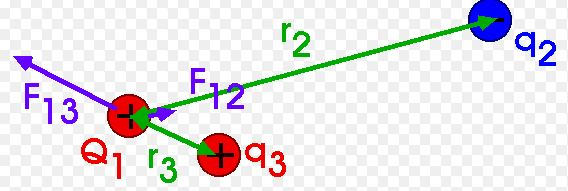
\includegraphics{3Force.JPG}
\end{figure}
Net force on $Q_{1}$:
\begin{equation*}
    \vec{F}_{T} = \vec{F}_{13} + \vec{F}_{12}
\end{equation*}
Using Coulomb's Law:
\begin{equation*}
    \vec{F}_{T} = k\Big[\frac{q_{1}q_{3}}{r_{13}^{2}}\hat{r}_{13} + \frac{q_{1}q_{2}}{r_{12}^{2}}\hat{r}_{12}\Big]
\end{equation*}
Generalising to n charges:
\begin{equation*}
    \vec{F}_{T} = \sum_{i = 1}^{n} \vec{F}_{i\,on\,0},~~n \in \mathbb{N}
\end{equation*}

\textbf{Example: }
\begin{table}[H]
    \begin{tabular}{|c|c|c|}
    \hline
    \rowcolor{lightgray} & Charge & Position Vector \\
    \hline
    $q_{0}$ & $-0.5\times10^{-9}$\,C & $\vec{r}_{0} = 5\,\text{cm}\hat{j}$\\
    \hline
    $q_{1}$ & $1\times10^{-9}$\,C & $\vec{r}_{1} = -0.1\,\text{cm}\hat{i}$\\
    \hline
    $q_{2}$ & $-1\times10^{-9}$\,C & $\vec{r}_{2} = 0.1\,\text{cm}\hat{i}$\\
    \hline
    \end{tabular}
\end{table}
Coulomb:
\begin{gather*}
    \vec{F}_{0} = k\Bigg[\frac{q_{1}q_{0}}{r_{10}^{2}}\hat{r}_{10} + \frac{q_{2}q_{0}}{r_{20}^{2}}\hat{r}_{20}\Bigg] \\
    \hat{r}_{10} = 0.1\hat{i} + 5\hat{j} ~~~~ \hat{r}_{20} = -0.1\hat{i} + 5\hat{j} \\
    |r_{10}| = |r_{20}| \approx 5\,\text{cm} \\
    \hat{r}_{10} = 0.02\hat{i} + \hat{j} ~~~~ \hat{r}_{20} = -0.02\hat{i} + \hat{j}
\end{gather*}
$q_{1}$ and $q_{2}$ act as an electric dipole
\begin{gather*}
    \vec{F}_{0} = k\frac{q_{1}q_{0}}{r_{10}^{2}}\Big[\hat{r}_{10} - \hat{r}_{20}\Big] \\
    ~~~~ = 9\times10^{9} \cdot \frac{1\times10^{-9}\times0.5\times10^{-9}}{25}\Big[4\times10^{-2}\hat{i}\Big] \\
    ~~~~ = -1.8\times10^{-6}\,N\,\hat{i}
\end{gather*}

\section{Electric Field}
A charge modigies properties of space around it, the modification being described by an electric field, $\vec{E}$ \\
Electric field describes the force per unit charge at a point in space due to a fixed charge
\begin{equation*}
    \vec{E} = \frac{\vec{F}}{q_{0}}
\end{equation*}
Units are N C$^{-1}$ \\
It is a vector field \\
Charges placed in an electric field experience $\vec{F} = q\vec{E}$ \\
$\vec{E}$ reacts instantaneously to the change in charge producing it \\
Superposition of electric field at a point of space means field addition is possible

\chapter{}
\section{Electric Field of a Point Charge}
Force on test charge, $q_{0}$, due to q:
\begin{gather*}
    \vec{F} = k\frac{q_{0}q}{|\mathbf{r}|^{2}} \mathbf{\hat{r}}, \\
    \because \vec{F} = \vec{E}q_{0} \implies \vec{E} = k\frac{q}{r^{2}}\hat{r}, \\ \therefore \vec{E} = \frac{q}{4\pi\epsilon_{0}r^{2}}\hat{r}
\end{gather*}
Electric field of a point charge is radial as it is always perpendicular to a spherical shell, with radius r, centered on the charge.

\begin{figure}[H]
    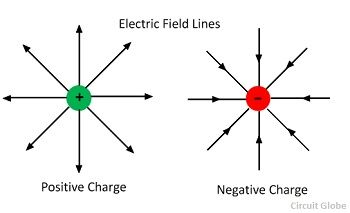
\includegraphics{electric-field-line.jpg}
\end{figure}

It is convenient to represent electric field in space using electric field lines. The bigger the separation, the snaller the magnitude of the electric field.

\section{Charge Distributions}
Need a convenient method of determining electric fields due to an arrangement or distribution of many charges on an object. \\
Key concept in this approach is the charge density, positive or negative.

\subsection{Linear Charge Distribution}
A charge, q, is evenly spread over a line of length, L. \\
Linear charge density with units of $C\,m^{-1}$:
\begin{equation*}
    \lambda = \frac{q}{L}
\end{equation*}

\subsection{Surface Charge Distribution}
Charge, Q, spread evenly over an area, A. \\
Surface Charge Density with units of $C\,m^{-2}$:
\begin{equation*}
    \sigma = \frac{Q}{A}
\end{equation*}

\subsection{Volume Charge Distribution}
Charge, Q, spread evenly over a volume, V. \\
Volume Charge Density with units of $C\,m^{-3}$:
\begin{equation*}
    \rho = \frac{Q}{V}
\end{equation*}
We can demonstrate the power of this approach with some examples.

\subsection{LCD -- Charged Ring}
Ring of radius, a, and charge, Q

\begin{figure}[H]
    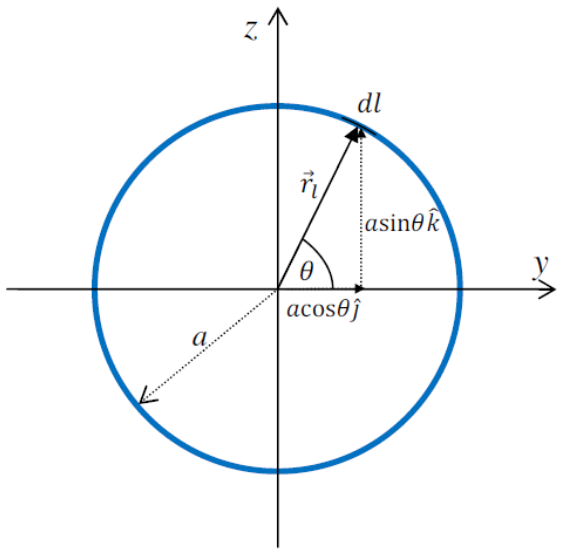
\includegraphics[scale=0.4]{Selection_004.png}
\end{figure}

A small length, dl, holds a charge, $dq = \lambda\,dl,~dl = a\,d\theta$

\begin{figure}[H]
    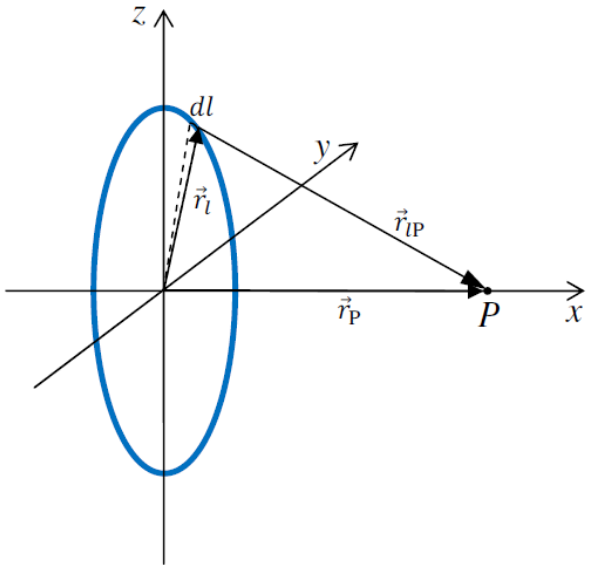
\includegraphics[scale=0.4]{D1.png}
\end{figure}

What is E at a point, P, at a distance, x, from the centre?
Put a test charge ar point P. \\
Determine the force due to dq on $q_{0}$.
\begin{gather*}
    d\vec{F}_{P} = \frac{kq_{0}dq}{r^{2}} \hat{r} = \frac{kq_{0}\lambda dl}{r^{2}} \hat{r} = \frac{kq_{0}\lambda a d\theta}{r^{2}} \hat{r} \\
    \vec{r}_{lP} = \vec{r}_{P} - \vec{r}_{l} = x \hat{i} - (a\cos\theta \hat{j} + a\sin\theta \hat{k}) \\
    \big|\vec{r}_{lP}\big| = \sqrt{\vec{r}_{lP} \cdot \vec{r}_{lP}} = \sqrt{x^{2} + a^{2}} \\
    \hat{r} = \frac{\vec{r}_{lP}}{|r|} = \frac{\vec{r}_{lP}}{\sqrt{x^{2} + a^{2}}} \\
    \implies d\vec{F}_{P} = \frac{k q_{0} a \lambda d\theta}{(x^{2} + a^{2})} \cdot \frac{\vec{r}_{lP}}{\sqrt{x^{2} + a^{2}}} \\
    \implies \vec{F}_{P} = \int_{0}^{2\pi} d\vec{F}_{P} = \frac{k q_{0} a \lambda}{(x^{2} + a^{2})^{3/2}} \int_{0}^{2\pi} (x \hat{i} - a\cos\theta \hat{j} - a\sin\theta \hat{k}) \; d\theta \\
    \implies \vec{F}_{P} = \frac{k q_{0} a \lambda}{(x^{2} + a^{2})^{3/2}} \big[x\theta \hat{i} - a\sin\theta \hat{j} + a\cos\theta \hat{k} \big]_{0}^{2\pi} = \frac{k q_{0} a \lambda}{(x^{2} + a^{2})^{3/2}} \cdot 2\pi x \hat{i} \\
    \implies \vec{F}_{P} = \frac{k q Q x \hat{i}}{(x^{2} + a^{2})^{3/2}} \\
    \implies \vec{E}_{P} = \frac{\vec{F}_{P}}{q_{0}} = \frac{k Q x}{(x^{2} + a^{2})^{3/2}} \hat{i} \\
    x >> a \implies \vec{E} = \frac{Q}{4\pi\epsilon_{0}x^{2}} \hat{i} \\
    x << a \implies \vec{E} = \frac{Q x}{4\pi\epsilon_{0}x^{2}} \hat{i} \\
    x = 0 \implies \vec{E} = 0
\end{gather*}

\chapter{}
\section{Surface Charge Distributiom -- Charged Disk}
\begin{figure}[H]
    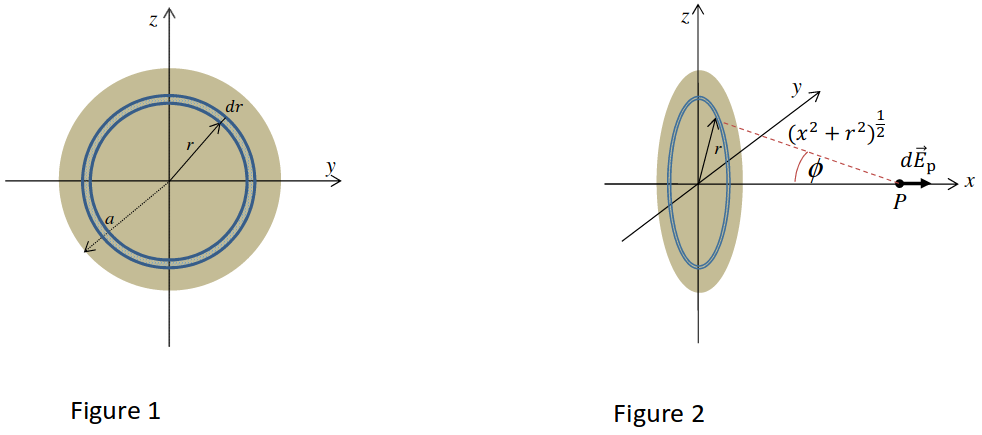
\includegraphics[scale=0.4]{R1.png}
\end{figure}
Look at circular sheet, radius a, with a charge, Q, evenly spread over it.

Surface Charge Density, $\sigma = \dfrac{Q}{\pi a^{2}}$

The disk can be considered to be made up of concentric rings of radius r, and thickness dr.

Charge on ring, $dq = \sigma \times \text{Area of ring} = \sigma \times 2\pi \, r \, dr$

What is E at Point P, a distance x along axis from O?

Field at P due to dq is:
\begin{gather*}
    d\vec{E} = \frac{k \, x \, dq}{(x^{2} + a^{2})^{3/2}} \hat{i} \\
    d\vec{E} = k \frac{x \sigma 2\pi r \, dr}{(x^{2} + a^{2})^{3/2}} \hat{i}
\end{gather*}
Total electric field at P is obtained by $\int_{0}^{a}$
\begin{equation*}
    \vec{E}_{P} = \int_{\text{disk}} d\vec{E}_{P} = \frac{k \sigma 2\pi}{x^{2}} \int_{0}^{a} \frac{r \, dr}{(1 + \tfrac{r^{2}}{x^{2}})^{3/2}} \hat{i}
\end{equation*}
Let $\dfrac{r}{x} = \tan\phi$, then $dr = x\sec^{2}\phi \, d\phi$ \\
Using $1 + \tan^{2}\phi = \sec^{2}\phi$, $\vec{E}_{P}$:
\begin{gather*}
    = k \sigma 2\pi \int \frac{\tan\phi \, \sec^{2}\phi}{\sec^{3}\phi} \hat{i} \, d\phi = k \sigma 2\pi \int \sin\phi \, d\phi \, \hat{i} \\
    = k \sigma 2\pi \big[-\cos\phi \big], ~~~~ \cos\phi = \frac{x}{\sqrt{x^{2} + r^{2}}} \\
    = -k \sigma 2\pi \Big[\frac{x}{\sqrt{x^{2} + r^{2}}} \hat{i} \Big]_{0}^{a} = k \sigma 2\pi \Big[\frac{x}{\sqrt{x^{2} + r^{2}}} \hat{i} \Big]_{a}^{0} \\
    = k \sigma 2\pi \Big[1 - \frac{x}{\sqrt{x^{2} + a^{2}}} \Big] \, \hat{i} = \frac{2 k Q}{a^{2}} \Big[1 - \frac{x}{\sqrt{x^{2} + a^{2}}} \Big] \, \hat{i}
\end{gather*}
\begin{gather*}
    x >> a \implies \vec{E} = \frac{2Qk}{x^{2}} \hat{i} \\
    x << a \implies \vec{E} = \frac{2Qk}{a^{2}} \hat{i} = \frac{Q}{2\pi \epsilon_{0} a^{2}} \hat{i} = \frac{\sigma}{2\epsilon_{0}} \hat{i}
\end{gather*}
i.e. $\vec{E}$ is uniform in space; it has the same magnitude and direction everywhere.

This leads to two parallel plates, oppositely charged, each with $|\sigma|$, can be used to deflect or accelerate charged particle beams.
Outside plates, the fields cancel; Inside plates, the fields add.

\subsection{Example:}
A proton of velocity $\bar{v} = 10^{3} \: m \, s^{-1} \; \hat{i}$ moves through a uniform electric field between parallel plates of $\vec{E} = -1 \times 10^{3} \; N \, C^{-1} \; \hat{k}$. \\
How far is the proton deflected in $t = 1 \mu s$? -- mass of proton $= 1.62 \times 10^{-27} kg$

Force, $\vec{F}_{p} = \vec{E}e$; $\vec{E}$ is uniform so force and acceleration are constant.
\begin{equation*}
    \vec{a}_{p} = \frac{\vec{F}_{p}}{m_{p}} = \frac{\vec{E}e}{m_{p}}
\end{equation*}
Using Newton \RN{2}:
\begin{equation*}
    \Delta z = \tfrac{1}{2}|\vec{a}_{p}|\epsilon^{2} = \tfrac{1}{2} \frac{|\vec{E}|e}{m_{p}}\epsilon^{2} = 0.05m
\end{equation*}

\section{Electric Flux}
Uniform field, $\vec{E}$, from a charged sheet. \\
Place a flat surface of area A parallel to charged sheet

Electric flux, $\Phi_{E} = |\vec{E}|A$, proportional to number of field lines intercepting the sheet. \\
If the flat surface is $\parallel$ to $\vec{E}$, $\Phi_{E} = 0$

\chapter{}
If the sheet is at some angle to the electric field, the vectors must be resolved:
\begin{gather*}
    \Phi_{E} = |\vec{E}|A\cos\theta \implies
    \Phi_{E} = \vec{E} \cdot \vec{A}
\end{gather*}
Vector Area, $\vec{A}$, perpendicular to flat surface:
\begin{equation*}
    \vec{A} = A\hat{n},
\end{equation*}
where $\hat{n}$ is a unit vector perpendicular to surface.

For a curved or non-uniform electric field, we use smaller vector areas, $d\vec{A}_{i}$: \\
Locally -- $\Phi_{E_{i}} = \vec{E} \cdot d\vec{A}_{i}$ \\
Total -- $\Phi_{E} = \sum_{i} \vec{E} \cdot d\vec{A}$ \\
As $d\vec{A} \to \infty$, $\Phi_{E} = \int \vec{E} \cdot d\vec{A}$ \\
This leads to Gauss' Law.

Total flux through closed surface is proportional to total charge inside closed surface. \\
Closed surface around charge is called Gaussian Surface (GS)

E.g. point charge, q: Choose GS to be spherical shell of radius r centered on the charge.
\begin{equation*}
    \Phi_{E} = \oint_{GS} \vec{E} \cdot d\vec{A}
\end{equation*}
Now each unit vector of area, $\vec{n}$, is $\parallel$ to $\vec{r}$ (electric field vector) and $\vec{E}$ is radial.
\begin{gather*}
    \Phi_{E} = \oint_{GS} |\vec{E}(r)| \vec{r} \; dA \, \vec{n} \\
    \Phi_{E} = |\vec{E}(r)| \oint_{GS} dA = |\vec{E}(r)|\, 4\pi r^{2} \\
    \implies = \frac{q}{4\pi\epsilon_{0}r^{2}}\, 4\pi r^{2} \\
    \implies = \frac{q}{\epsilon_{0}}
\end{gather*}

\subsection{Gauss' Law}
\begin{equation*}
    \Phi_{E} = \oint_{GS} \vec{E} \cdot d\vec{A} = \frac{Q}{\epsilon_{0}},
\end{equation*}
where Q is the charge enclosed by the Gaussian Surface.

\subsection{Example}
Uniformly charged (infinite) hollow cylinder of radius, R. \\
$\vec{E}$ is perpendicular to the surface. \\
Choose a GS which is cylindrical with radius, r, and length, l.

For $r > R$:
\begin{gather*}
    \oint_{GS} \vec{E} \cdot d\vec{A} = \frac{Q}{\epsilon_{0}} = \frac{\sigma \times \text{Area in GS}}{\epsilon_{0}} = \frac{\sigma 2\pi r l}{\epsilon_{0}} \\
    \Phi_{E} = \cancel{\oint_{end} \vec{E} \cdot d\vec{A}_{E}} + \oint_{side} \vec{E} \cdot d\vec{A}_{S} = \frac{\sigma 2\pi R l}{\epsilon_{0}}
\end{gather*}
\begin{gather*}
    |\vec{E}| \oint_{s} dA_{s} = |\vec{E}| 2\pi r l = \frac{\sigma 2\pi R l}{\epsilon_{0}} \\
    |\vec{E}| = \frac{\sigma R}{r \epsilon_{0}} \\
    \vec{E} = \frac{\sigma R}{r \epsilon_{0}} \; \hat{r}
\end{gather*}
If $r < R$, there is no enclosed charge, $\therefore \vec{E} = 0$.

\chapter{}
\section{Uniformly charged (infinite) hollow cylinder, radius R, continued}

For a plot of $|\vec{E}|$ against r, $|\vec{E}|$ is 0 for $r < R$, equal to $\frac{\sigma}{\epsilon_{0}}$ at $r = R$, and then decreases from there as r increases $\propto \frac{1}{r^{2}}$.

\subsection{Example:}
Solid, uniformly charged sphere, radius R, charge q

Volume charge density:
\begin{equation*}
    \rho = \frac{q}{V} = \frac{3q}{4\pi r^{3}}
\end{equation*}
Choose a GS which is a spherical shell with radius, r. \\
Use Gauss' Law.

For $r > R$:
\begin{equation*}
    \Phi_{E} = \oint \vec{E} \cdot d\vec{A} = \frac{q}{\epsilon_{0}}
\end{equation*}
For $\hat{n} \parallel \hat{r}$,
\begin{equation*}
    \oint |\vec{E}| \hat{r} \cdot dA \, \hat{n} = \oint |\vec{E}|dA = \frac{q}{\epsilon_{0}}
\end{equation*}
This is a radial problem so $|\vec{E}|$ is the same at constant radius.
\begin{gather*}
    |\vec{E}| \oint dA = \vec{E} 4\pi r^{2} = \frac{q}{\epsilon_{0}} \\
    |\vec{E}| = \frac{q}{4\pi\epsilon_{0}r^{2}} \\
    \vec{E} = \frac{q}{4\pi\epsilon_{0}r^{2}} \, \hat{r}
\end{gather*}
For $r < R$:
\begin{equation*}
    Q = \rho \times V = \tfrac{4}{3}\rho\pi r^{3}
\end{equation*}
As above, $\hat{n} \parallel \hat{r}$ so:
\begin{gather*}
    |\vec{E}| \oint dA = |\vec{E}| \cancel{4\pi r^{2}} = \frac{\rho \cancel{4\pi}r^{\cancel{3}}}{3\epsilon_{0}} \\
    \vec{E} = \frac{\rho r}{3\epsilon_{0}} = \frac{\cancel{3}q}{4\pi R^{3}} \times \frac{r}{\cancel{3}\epsilon_{0}} = \frac{qr}{4\pi \epsilon_{0} R^{3}}
\end{gather*}

\section{Charges on Conductors}
Excess charge on conductor resides on the surface. \\
The interior of the conductor has $\vec{E} = 0$ as electrons arrange themselves to shield the interior, regardless of whether it is hollow or solid.

Place charge, q, in center of hollow cavity. \\
Charge rearranges to maintain $\vec{E} = 0$, electrons move from or to the outer surface to produce shielding. \\
Use Gauss' Law; Choose spherical GS

$r > R_{s}$:
\begin{gather*}
    \Phi_{E} = \oint \vec{E} \cdot d\vec{A} \\
    \Phi_{E} = |\vec{E}| \; 4\pi r^{2}= \frac{Q_{i} + q}{\epsilon_{0}} \\
    \therefore \vec{E} = \frac{Q_{i} + q}{4\pi \epsilon_{0} r^{2} }
\end{gather*}
$R_{H} < r < R_{s}$:
\begin{equation*}
    Q_{encl} = 0 \to \vec{E} = 0
\end{equation*}
$R_{H} > r$:
\begin{equation*}
    Q_{encl} = q \to \vec{E} = \frac{q}{4\pi \epsilon_{0} r^{2}} \, \hat{r}
\end{equation*}

\chapter{}
\section{Electric Potential Energy, U}
Consider work done by the electric force due to a point charge, q, on a charge, $q_{0}$.
\begin{equation*}
    \vec{F} = k \frac{q_{0} q}{r^{2}} \; \hat{r}
\end{equation*}
Work done by electric force when moving $q_{0}$ a distance, dr:
\begin{equation*}
    \vec{F} \cdot d\vec{l} = q_{0}\vec{E} \cdot d\vec{l}, ~~~ d\vec{l} = dr \cdot \hat{r}
\end{equation*}
Total work done when moving $q_{0}$ from $r_{a}$ to $r_{b}$:
\begin{gather*}
    W_{a \to b} = \int_{a}^{b} \vec{F} \cdot d\vec{l} = q_{0} \int_{a}^{b} \vec{E} \cdot d\vec{l} \\
    W_{a \to b} = k q_{0} q \int_{a}^{b} \frac{1}{r^{2}} \; dr = k q_{0} q \Big[\frac{1}{r_{a}} - \frac{1}{r_{b}} \Big]
\end{gather*}
Note: The electric force is a conservative force -- work done can be described by a change in potential energy. \\
For an electric force acting on a charge, $W_{a \to b} = U_{a} - U_{b}$.
\begin{gather*}
    U = k \frac{q_{0} q}{r}, ~~
    \begin{cases}
        > 0 & \text{if like charges} \\
        < 0 & \text{if opposite charges}
    \end{cases}
\end{gather*}
From the principle of superposition of forces and fields, the potential energy due to more than one charge:
\begin{gather*}
    U = kq_{0}\Big[\frac{q_{1}}{r_{1}} + \frac{q_{2}}{r_{2}} \Big]\\
    U = kq_{0} \sum_{i} \frac{q_{i}}{r_{i}}
\end{gather*}

\section{Electric Potential, V}
\begin{equation*}
    V = \frac{U}{q_{0}}
\end{equation*}
Unit: Volt, V -- $1\;V = 1\;J\,C^{-1}$
\begin{gather*}
    W_{a \to b} = U_{a} - U_{b} = q_{0} \big(V_{a} - V_{b}\big) \\
    \frac{W_{a \to b}}{q} = V_{a} - V_{b} ~~~ \text{-- Potential Difference (p.d.)} \\
    V =
    \begin{cases}
        \frac{U}{q_{0}} = \frac{kq}{r} & \text{for a single charge} \\
        k \sum_{i} \frac{q_{i}}{r_{i}} & \text{for a collection of charges}
    \end{cases} \\
    \Delta V = \int_{r_{1}}^{r_{2}} \vec{E} \cdot d\vec{l}
\end{gather*}
Can find p.d. if $\vec{E}$ is known and vice versa.

\chapter{}
Recall:
\begin{equation*}
    V = \frac{U}{q_{0}} = k \sum_{i} \frac{q_{i}}{r_{i}}
\end{equation*}
For a continuous charge distribution over a body, divide charge into elements, dq, and convert sum to integral:
\begin{equation*}
    V = k \int \frac{dq}{r}
\end{equation*}
Use this result to compute V without knowledge of $\vec{E}$.

\subsection{Example:}
Uniformly charged ring with charge, Q, and radius, a. \\
Linear charge density of $\lambda = \frac{Q}{2\pi a}$.
\begin{gather*}
    dq = \lambda dl = \lambda a d\theta \\
    V_{x} = k \int \frac{dq}{r} = k \int \frac{\lambda a d\theta}{\sqrt{x^{2} + a^{2}}} \\
    V_{x} = \frac{k\lambda a}{\sqrt{x^{2} + a^{2}}} \int_{0}^{2\pi} d\theta = \frac{k2\pi a \lambda}{\sqrt{x^{2} + a^{2}}} \\
    \textbf{Note: } \lim_{x \to \infty} V = 0 \\
    V = \frac{kQ}{\sqrt{x^{2} + a^{2}}} ~~~ \because 2\pi a \lambda = Q
\end{gather*}
\textbf{Note:} Calculation with V often avoids complications of vector analysis used when determining $\vec{E}$. We can determine $\vec{E}$ from V.
\begin{gather*}
    V_{a} - V_{b} = - \int_{b}^{a} dV = - \int_{b}^{a} \vec{E} \cdot d\vec{l} \\
    \implies dV = - \vec{E} \cdot d\vec{l}
\end{gather*}
Say $\vec{E}$ and $d\vec{l}$ are aligned:
\begin{gather*}
    \vec{E} \cdot d\vec{l} = E_{x}dx \\
    \implies E_{x} = - \frac{dV}{dx}
\end{gather*}
$E_{x}$ is the \emph{potential gradient}.

In general, $\vec{E}$ and V vary in all directions:
\begin{gather*}
    E_{x} = - \frac{\partial V}{\partial x}, ~~~ E_{y} = - \frac{\partial V}{\partial y}, ~~~ E_{z} = - \frac{\partial V}{\partial z} \\
    \vec{E} = - \Bigg(\frac{\partial V}{\partial x} \hat{i} + \frac{\partial V}{\partial y} \hat{j} + \frac{\partial V}{\partial z} \hat{k} \Bigg) = - \vec{\nabla} V
\end{gather*}
Back to 1D ring:
\begin{gather*}
    V = \frac{kQ}{\sqrt{x^{2} + a^{2}}} \\
    \vec{E} = -\vec{\nabla}V = - \frac{\partial V}{\partial x} \hat{i} \\
    \vec{E} = -kQ \frac{\partial}{\partial x} \Bigg[\frac{1}{\sqrt{x^{2} + a^{2}}} \Bigg] \hat{i} = \frac{kQx}{(x^{2} + a^{2})^{3/2}} \hat{i}
\end{gather*}

\section{Equipotentials}
Consider the example of a uniformly charged hollow sphere of radius R. \\
For $r > R$:
\begin{gather*}
    \vec{E} = \frac{kQ}{r^{2}} \hat{r} \\
    V_{a} - V_{b} = \int_{r_{a}}^{r_{b}} \vec{E} \cdot d\vec{l} = \int_{r_{a}}^{r_{b}} \vec{E} \cdot d\vec{r} \\
    V_{a} - V_{b} = kQ \int_{r_{a}}^{r_{b}} \frac{dr}{r^{2}} = kQ \Big[ \frac{1}{r_{a}} - \frac{1}{r_{b}} \Big] \\
    \lim_{r_{b} \to \infty} V_{b} = 0 \\
    V_{a} = \frac{kQ}{r_{a}}
\end{gather*}
For $r < R$:
\begin{gather*}
    \vec{E} = 0 \\
    W_{a \to b}= q_{0}\big(V_{a} - V_{b} \big) \\
    \therefore V_{a} = V_{b} = \frac{kQ}{R} ~~[\text{everywhere inside the sphere}] \\
    V \propto \frac{1}{r} ~~[\text{outside sphere}]
\end{gather*}

\chapter{}
\subsection{Example:}
Electron starts at rest at the surface of a uniformly charged spherical shell of potential, $V = -1.0\,V$. \\
What is the maximum velocity attained by the electron?
Maximum velocity is at $r = \infty$ and $V_{b} = 0$.
\begin{gather*}
    W_{a \to b} = q_{0} \big(V_{a} - V_{b} \big) = \tfrac{1}{2}m_{e}\vec{v}^{2} \\
    \vec{v} = \sqrt{\frac{2q_{0}V_{a}}{m_{e}}} \hat{r} = \big(5.9 \times 10^{5} \; m\,s^{-1} \big) \hat{r}
\end{gather*}

\section{Capacitance}
A body with charge, Q, has a potential, V, with respect to $V(r = \infty) = 0$. \\
Alternative view: The body has a capacity to hold a charge, Q, when at potential, V. Quantify this capacity as capacitance:
\begin{equation*}
    C = \frac{Q}{V}
\end{equation*}
At surface of sphere, radius R, charge Q:
\begin{equation*}
    V = \frac{Q}{4\pi\epsilon_{0} R} \implies C = \frac{Q}{V} = 4\pi\epsilon_{0}R
\end{equation*}
e.g. spherical Van de Graaf dome:
\begin{gather*}
    R \approx 9.5 \; cm \\
    C = 11 \times 10^{-12} \; F\,[C\,V^{-1}] = 11 \; pF \\
    V \approx + 35\;V \\
    Q = VC \approx 3.7 \times 10^{-10} \; F
\end{gather*}
A device which stores charge and energy is a \emph{Capacitor}.

e.g. Parallel plate capacitor: \\
Area of plate, A
\begin{gather*}
    V_{a} - V_{b} = |\vec{E}|d \\
    \vec{E} \frac{V_{a} - V_{b}}{d}
\end{gather*}
Recall that the uniform electric field has the form, $|\vec{E}| = \frac{\sigma}{\epsilon_{0}}$. \\
This was for infinite plates, but the expressions is good when $A >> d$.
\begin{gather*}
    \sigma = \frac{Q}{A} \implies V_{a} - V_{b} = \frac{\sigma d}{\epsilon_{0}} = \frac{Q d}{A \epsilon_{0}} \\
    C = \frac{Q}{V_{a} - V_{b}} = \frac{A \epsilon_{0}}{d}
\end{gather*}
Conventional capacitors are often based on concentric cylindrical plates, small radius a, large radius b

Assume $d >> a,\,b$ and use the results from lecture 5 where we used Gauss' Law to show that, for radius $r > a$:
\begin{gather*}
    \vec{E} \frac{\sigma a}{\epsilon_{0} r} \hat{r} \\
    \sigma = \frac{Q}{2\pi a l} \implies \\
    \vec{E} = 2\pi \epsilon_{0} l r \hat{r} \\
    V_{a} - V_{b} = \int_{a}^{b} \vec{E} \cdot d\vec{r} = \int_{a}^{b} \frac{Q}{2\pi\epsilon_{0}lr}\,dr \\
    V_{a} - V_{b} = \frac{Q}{2\pi\epsilon_{0}l}\Big[\ln\frac{b}{a}\Big] \\
    C = \frac{Q}{V_{a} - V_{b}} = \frac{2\pi\epsilon_{0}l}{\ln\tfrac{b}{a}}
\end{gather*}

\section{Equivalent Capacitance}
For parallel capacitors, the equivalent capacitance, $C_{p} = \sum_{i} C_{i}$

\chapter{}
p.d. across all capacitors in a parallel circuit is $V_{a} - V_{b}$, total charge is Q.
\begin{gather*}
    C_{1} = \frac{q_{1}}{V_{a} - V_{b}}, ~~ C_{2} = \frac{q_{2}}{V_{a} - V_{b}}, ~~ C_{3} = \frac{q_{3}}{V_{a} - V_{b}} \\
    Q = q_{1} + q_{2} + q_{3} = \big(V_{a} - V_{b} \big) \big(C_{1} + C_{2} + C_{3} \big) \\
    C_{p} = \frac{Q}{V_{a} - V_{b}} = C_{1} + C_{2} + C_{3} = \sum_{i} C_{i}
\end{gather*}
For capacitors in series:
\begin{gather*}
    V_{a} - V_{23} = \frac{q}{C_{3}}, ~~ V_{23} - V_{12} = \frac{q}{C_{2}}, ~~ V_{12} - V_{b} = \frac{q}{C_{1}} \\
    V_{a} - V_{b} = \big(V_{a} - V_{23} \big) + \big(V_{23} - V_{12} \big) + \big(V_{12} - V_{b}\big) \\
    V_{a} - V_{b} = q \Big[\frac{1}{C_{3}} + \frac{1}{C_{2}} + \frac{1}{C_{1}} \Big] \\
    \frac{V_{a} - V_{b}}{q} = \frac{1}{C_{s}} = \Big[\frac{1}{C_{3}} + \frac{1}{C_{2}} + \frac{1}{C_{1}} \Big] \\
    \frac{1}{C_{s}} = \sum_{i} \frac{1}{C_{i}} \\
    C_{s} = \frac{1}{\sum_{i} \tfrac{1}{C_{i}}}
\end{gather*}

\section{Insulators in an electric field}
A polarised insulator consists of an electric dipole (permanently induced) \\
Insulator is put into gap of a parallel plate capacitor, capacitance $C_{0}$
\begin{equation*}
    C_{0} = \frac{Q}{V_{0}} \to C = \frac{Q}{V}
\end{equation*}
\begin{figure}[H]
    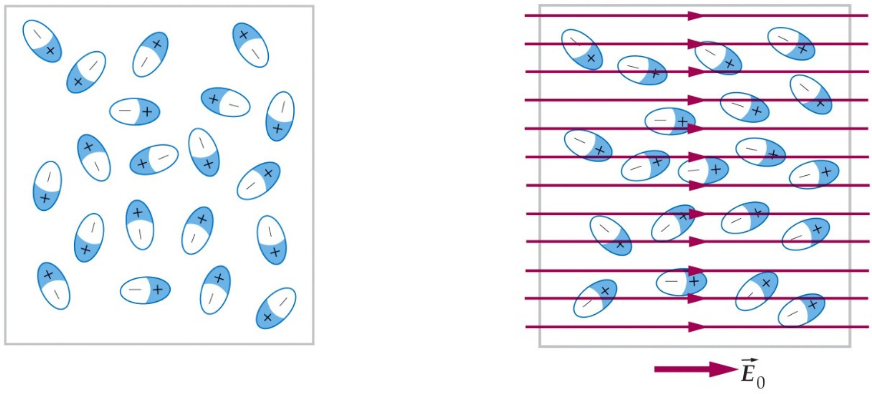
\includegraphics[scale=0.4]{Diploes.png}
\end{figure}
Insulator is polarised by the electric field. \\
This is a relatively weak effect and the induced charge densities at the surfaces, $\sigma_{i}$ (bound charges) is much smaller than (free) charge densities on the parallel plates, $\pm \sigma$. \\
Induced charges produce an electric field which opposes the applied field.

Use Gauss' Law to determine the new total electric field, choose cubic GS:
\begin{gather*}
    \Phi_{E} = \oint \vec{E} \cdot d\vec{A} = \frac{(\sigma - \sigma_{i})dA}{\epsilon_{0}} \\
    \vec{E} = E_{x} \hat{i} \\
    |\vec{E}| dA = \frac{(\sigma - \sigma_{i})dA}{\epsilon_{0}} \\
    |\vec{E}| = \frac{\sigma - \sigma_{i}}{\epsilon_{0}} \\
    \vec{E} = \frac{\sigma}{K \epsilon_{0}} = \frac{|\vec{E}|}{K} \\
    \sigma_{i} = \sigma \Big(1 - \frac{1}{K} \Big)
\end{gather*}
$K :=$ Dielectric constant or relative permitivity

\chapter{}
\section{Insulators in parallel plate capacitors}
\begin{gather*}
    V = V_{a} - V_{b} = \int_{a}^{b} \vec{E} \cdot d\vec{l} = \frac{1}{K} \int_{a}^{b} \vec{E}\cdot d\vec{l} = \frac{V_{0}}{K} \\
    C_{0} = \frac{Q}{V_{0}} = \frac{\epsilon_{0} A}{d} \\
    C = \frac{Q}{V} = \frac{KQ}{V_{0}} = \frac{K\epsilon_{0}A}{d} ~~ \Big/ ~~ C = \frac{\epsilon A}{d} \\
    \epsilon = K\epsilon_{0} := \text{absolute permitivity of insulator}
\end{gather*}
Note: In general, we replace $\epsilon_{0}$ with $\epsilon$ when filling a capacitor with an insulator.

e.g. Cylindrical capacitor:
\begin{equation*}
    C = \frac{2\pi\epsilon l}{\ln\tfrac{b}{a}}
\end{equation*}

\subsection{Example:}
Find $C_{E}$ in terms of $C_{0} = \frac{\epsilon_{0}A}{d}$.
\begin{figure}[H]
    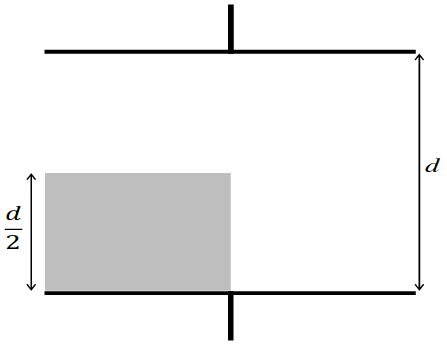
\includegraphics[scale=0.5]{Cap2.png}
\end{figure}
Using Gauss' Law, it can be shown that the capacitor can be replaced with three different capacitors: two on the left for the to and bottom sections, $C_{1}$ and $C_{2}$, and one for the right, $C_{3}$.
\begin{gather*}
    C_{1} = \frac{\epsilon_{0}\tfrac{A}{2}}{\tfrac{d}{2}}, ~~~ C_{2} = \frac{\epsilon_{0}K\tfrac{A}{2}}{\tfrac{d}{2}}, ~~~ C_{3} = \frac{\epsilon_{0}\tfrac{A}{2}}{d} \\
    C_{LHS}: \frac{1}{C_{LHS}} = \frac{1}{C_{1}} + \frac{1}{C_{2}} = \frac{d}{\epsilon_{0}} \Big[1 + \frac{1}{K}\Big] \\
    C_{LHS} = \frac{\epsilon_{0}KA}{d(K + 1)} \\
    C_{E} = C_{LHS} + C_{3} = \frac{\epsilon_{0}A}{2d} + \frac{\epsilon_{0}KA}{d(K + 1)} = \frac{\epsilon_{0}A}{d}\Big[\frac{3K + 1}{2(K + 1)}\Big] \\
    \frac{C_{E}}{C_{0}} = \frac{3K + 1}{2(K + 1)}
\end{gather*}

\section{Potential Energy Stored In A Capacitor}
\begin{equation*}
    C = \frac{q}{V_{a} - V_{b}} = \frac{q}{V}
\end{equation*}
Work done against electric field by the battery in moving a small charge, dq, from b to a:
\begin{equation*}
    dW = dq\big(V_{a} - V_{b}\big) = dq \cdot V = \frac{q}{C}dq
\end{equation*}
Total work done to charge capacitor from 0 to Q:
\begin{equation*}
    W = \int dW = \int_{0}^{Q} \frac{q}{C} dq = \tfrac{1}{2} \frac{Q^{2}}{C} = \tfrac{1}{2}CV^{2}
\end{equation*}
As work done increases, potential energy (PE) does too. Initial PE, $U_{i} = 0$; final PE, $U_{f} = U$.
\begin{equation*}
    W = U_{f} - U_{i} = U = \tfrac{1}{2}\frac{Q^{2}}{C} = \tfrac{1}{2}CV^{2}
\end{equation*}
Define potential energy density, u = PE per unit volume.
\begin{equation*}
    u = \tfrac{1}{2}\epsilon_{0}|\vec{E}|^{2}
\end{equation*}
This holds true for any electric field configuration.

\section{Electrostatics}
The flow of movement of charge. \\
A p.d. acts to do work on a charge, moving it from a lower potential to a higher potential. \\
Flow of charge is represented by the electric current, I.
\begin{equation*}
    I = \frac{dQ}{dt} := \text{net charge moving through an area per unit time}
\end{equation*}
Unit -- Amperes/Amps (A) $= C\,s^{-1}$ \\
Conventional current flows in a direction where there is a flow of positive charge. \\
Charge is 'resisted' by the conductor (wire), otherwise I tends to $\infty$, and the property of conductors which resists charge flow is the resistance, R. \\
Ohm's Law:
\begin{equation*}
    V = V_{a} - V_{b} = IR
\end{equation*}
Unit -- Ohm ($\Omega$) $= V\,A^{-1}$
\begin{equation*}
    R = \frac{\rho l}{A}
\end{equation*}
$\rho$ - Resistivity := property of material; limited bby charge scattering due to atomic vibrations and defects in material. \\
Conductivity := $\frac{1}{\rho}$

\chapter{}
\section{Electromotive Force, $\varepsilon$, EMF}
Unit, Volt, V \\
EMF is the property of a battery or other device which 'pumps' charge from low to high potential in a closed circuit. \\
Work done on a charge, q, by EMF is $q\varepsilon$. \\
Ideal EMF source provides a constant p.d. regardless of current.

\section{Electric Power}
In time, dt, a charge, $dQ = I\,dt$, passes through a circuit element (CE) \\
PE change:
\begin{equation*}
    U_{i} = dQ\,V_{a}, ~~ U_{f} = dQ\,V_{b}
\end{equation*}
Work done in moving charge through CE:
\begin{gather*}
    W_{a \to b} = U_{i} - U_{f} = \big(V_{a} - V_{b} \big)dQ \\
    W_{a \to b} = I\big(V_{a} - V_{b} \big)dt
\end{gather*}
Rate of energy delivery to CE is the electrical power, P -- units of Watts (W) := $J\,s^{-1}$
\begin{gather*}
    P = I\big(V_{a} - V_{b} \big) = IV \\
    P = IV = I^{2}R = \frac{V^{2}}{R}
\end{gather*}
Note: sources of EMF are not perfect and have an internal resistance, r \\
True p.d. across terminals of a battery is:
\begin{equation*}
    V = \varepsilon - Ir
\end{equation*}
Power from a battery:
\begin{equation*}
    P = IV = \varepsilon I - I^{2}r
\end{equation*}
The first term is the rate at which work is done on circulating charge, and the second is energy dissipating in the battery.

e.g. Car battery:
\begin{gather*}
    \varepsilon = 12.6 \; V \\
    r = 0.005 \; \Omega \\
    I_{start} \approx 120 \; A \\
    P = 1.5 \; kW,~\text{lost 72 W in r}
\end{gather*}

\section{Electrical Circuits -- Kirchoff's Rules}
\begin{enumerate}
    \item The algebraic su, of currents arriving at any junction in the circuit is zero: $\sum_{i} I_{i} = 0$
    \item The sum of p.d.s around any closed loop of a circuit network is zero: $\sum_{i} V_{i} = 0$
\end{enumerate}

\part{Magnetism}
\chapter{}
\subsubsection{Lectures for this part of the course were very poor -- refer heavily to textbook}

Force of interaction between magnetic poles:
\begin{equation*}
    F \approx \frac{p_{1}p_{2}}{d^{2}}
\end{equation*}
$p_{1}$ and $p_{2}$ are the magnetic pole strengths

An electric charge has an electric field and also a magnetic field when \emph{in motion} \\
Magnetic field is a relativistic by-product of Electromagnetism

Electric charge is relativistically invariant; magnetic field is associated with relative motion of the charge to observer -- $v = 0 \implies B = 0$

In bar magnets, motion is in the electrons of the atoms, which are in constant motion. \\
There are two motions:
\begin{enumerate}
    \item electron spin
    \item electron revolution
\end{enumerate}
Electron spin is the most common cause of magnetism

\section{Force on a moving charge}
The force acting on a charge, q, moving with velocity, v, through a magnetic field with flux denisty, $\vec{B}$, is given by:
\begin{equation*}
    \vec{F} = q\vec{v} \times \vec{B}, ~ \vec{F} \perp \vec{B}
\end{equation*}
$\vec{B}$ -- magnetic field density \\
$\vec{H}$ -- magnetic field strength

Con combine electric and magnetic forces into \emph{the Lorentz force:}
\begin{equation*}
    \vec{F} = q \big( \vec{E} + \vec{v} \times \vec{B} \big)
\end{equation*}
$\vec{F} \neq q\vec{B}$ as there are no magnetic monopoles

$\odot$ -- $\vec{B}$ is coming out of the page \\
$\otimes$ -- $\vec{B}$ is going into the page
\begin{equation*}
    |F_{B}| = |q||\vec{v}||\vec{B}|\sin\theta
\end{equation*}
\begin{itemize}
    \item[$\vec{E}$ --] Change KE, -ve or +ve, does work
    \item[$\vec{B}$ --] does no work, $\perp$, can change direction of motion but not KE
    \item[$\vec{B}$ --] has units, Tesla, T, $N\,A^{-1}\,m^{-1}$
\end{itemize}

\chapter{}
Charged particle, +ve q, B field parallel
\begin{gather*}
    F_{B} = q\big(\vec{v \times \vec{B}} \big)\\
    F_{B} = qvB = \frac{mv^{2}}{r} \\
    R = \frac{mv}{qB}
\end{gather*}
Helical path for $\cancel{\perp}$
\begin{equation*}
    \vec{F} = "\vec{I}" \times \vec{B}
\end{equation*}
*\textit{Current is not actually a vector}

\textbf{SEE TEXTBOOK FOR REST OF MAGNETISM -- LECTURES BECOME IMCOMPREHENSIBLE AT THIS POINT}






























































\end{document}
